
\section{Umfrage}
Im Rahmen der Projektvorbereitung sollte auch eine Umfrage unter potenziellen Kunden erfolgen. So sollen möglichst früh in der Entwicklung Wünsche und die Sicht der Kunden auf ein Produkt oder ein Problem eingeholt werden. Hierbei handelt es sich um den sogenannten Customer Insight, welcher uns neue Perspektiven eröffnen soll. Damit soll verhindert werden, dass wir in unseren Ideen möglicherweise etwas ganz Entscheidendes vergessen, was aber aus der Sicht der Kunden besonders wichtig ist. Es sollen außerdem auch möglichst viele verschiedene Anforderungen der einzelnen Personen erhalten werden. Dafür haben wir eine Umfrage mit insgesamt 19 Fragen entwickelt. Am Ende konnten wir immerhin 44 Teilnehmende aufweisen.
\\
\\
Zuerst kamen ein paar Fragen zum Fahrzeug der Teilnehmer, z.B. von welcher Marke und wie alt es ist. Im zweiten Abschnitt stellten wir einige Fragen zur Sicherheit der Fahrzeuge der Teilnehmer, z.B. wie sie gegen Diebstahl geschützt sind und ob schon einmal etwas gestohlen wurde. Als nächstes folgten Fragen, mit denen wir direkte Bedürfnisse und Anforderungen für unser Produkt herausfinden wollten, unter anderem wurde gefragt, was ihn/sie an aktuell zu erwerbenden Autoalarmsystemen stört und wieviel er/sie maximal für ein solches System ausgeben würde. Zum Abschluss wurden noch ein paar persönliche Informationen für mögliche statistische Zusammenhänge abgefragt, wie Geschlecht, Alter und Beschäftigungsverhältnis.
Konkret setzte sich die Umfrage aus folgenden Fragen zusammen:

\begin{itemize}
	\item Von welcher Marke ist dein Auto?
	\item Zu welcher Fahrzeugklasse gehört dein Auto?
	\item Welches Baujahr ist dein Auto?
	\item Wie teuer war dein Auto ungefähr und wieviel ist es jetzt noch wert?
	\item Wie wichtig ist dir dein Auto? (Emotionale Bindung usw.)
	\item Wie ist dein Auto gegen Einbruch und Diebstahl geschützt?
	\item Wie zufrieden bist du mit deiner Sicherheitslösung?
	\item Wurde dir bereits ein Auto geklaut oder es versucht?
	\item Wurde schon einmal in dein Auto eingebrochen oder es versucht?
	\item Wenn ja, was wurde geklaut?
	\item Wie ist dein Auto versichert?
	\item Wo parkst du dein Auto normalerweise?
	\item Um was hast du Angst, wenn dein Auto unbeaufsichtigt ist?
	\item Was stört dich an bisher käuflich erwerblichen Alarmsystemen für Autos bzw. was würdest du an diesen ändern?
	\item Wie viel würdest du für ein neues Alarmsystem für dein Auto ausgeben?
	\item Du bist... (männlich, weiblich, divers)
	\item Wie alt bist du?
	\item Wie ist dein derzeitiges Beschäftigungsverhältnis?
	\item Wie hoch ist dein monatliches Nettoeinkommen?
\end{itemize}
Die Umfrage wurde mit Hilfe von Google Forms realisiert und ist noch unter folgendem Link abrufbar: https://forms.gle/qNTWM4qkF7ykG4tt9

\section{Persona} 
Des Weiteren sollte die Frage geklärt werden: Wie kann die Fähigkeit, sich in andere Personen hineinversetzen zu können, ihre Bedürfnisse und Motivation nachzuvollziehen und Verhaltensmuster vorherzusagen, zur Zielgruppenanalyse genutzt werden? \cite{JosefineLepzien} Nachfolgend stellen wir kurz unsere Persona vor, welche wir auf Basis der Auswertung der im vorherigen Abschnitt erläuterten Umfrage  konzipiert und charakterisiert haben. 

\begin{figure} [H]
	\begin{center}
		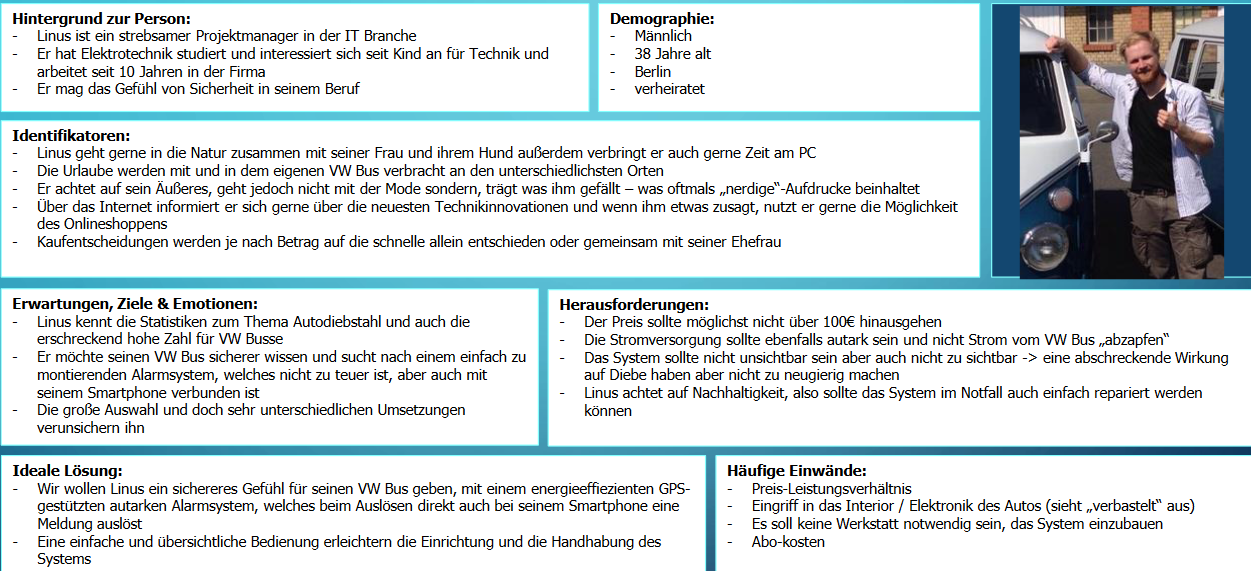
\includegraphics[width=1\textwidth]{Bilder/Konzept_Persona.png}
		\caption{Persona \textit{Linus Schrödinger}}
		\label{persona}
	\end{center}
\end{figure}
Unsere Persona namens Linus Schrödinger ist zusammenfassend gesagt, ein technikinteressierter naturbegeisterter Ehemann, der es liebt mit seiner Frau und seinem VW Bus zu verreisen. Er mag das Gefühl von Sicherheit und ist daher beunruhigt über die hohe Anzahl der Autodiebstähle allein für VW Busse - ein nachrüstbares Alarmsystem stellt an sich heutzutage kein Problem mehr da, jedoch ist die Auswahl groß und verunsichern ihn in seiner Kaufentscheidung. Ihm ist wichtig, dass das System möglichst nachhaltig aufgesetzt ist, nicht in die eigentliche Fahrzeugelektronik eingreift und leicht selbst montiert werden kann.
\\
Ziel dieser Methode ist die Entwicklung von Nutzermodellen, die Personen einer spezifischen Zielgruppe mit bestimmten Merkmalen charakterisieren. Anhand einer generierten Persona kann vorausgesagt werden, was ein Charakter in bestimmten Situationen tun würde. \cite{JosefineLepzien}
\\
\\
Diese Persona stellt also einen fiktiven Charakter dar, der stellvertretend für einen Käufer unseres Alarmsystems steht. Ein solch imaginäres Modell half uns, sich in die Lage eines Kunden während der Entwicklung unseres Prototypen zu versetzen. Des Weiteren trägt die Auseinandersetzung dazu bei, sich mit konkreten Erwartungen, Zielen und Bedürfnissen des zukünftigen Kunden zu beschäftigen und unser System möglichst effizient und effektiv auf die von uns gewünschte Zielgruppe auszurichten.


\section{Konzept} 
Nachdem wir mit Hilfe der Umfrage und der Persona schon einen groben Eindruck bekommen haben, auf welche Zielgruppe unser Produkt passen könnte und welche Eigenschaften und Funktionen es erfüllen soll, erstellten wir ein erstes Konzept. Dieses Konzept beinhaltet alle wesentlichen Komponenten unseres Produkts und ist in der folgenden Abbildung schematisch dargestellt.
\begin{figure} [H]
	\begin{center}
		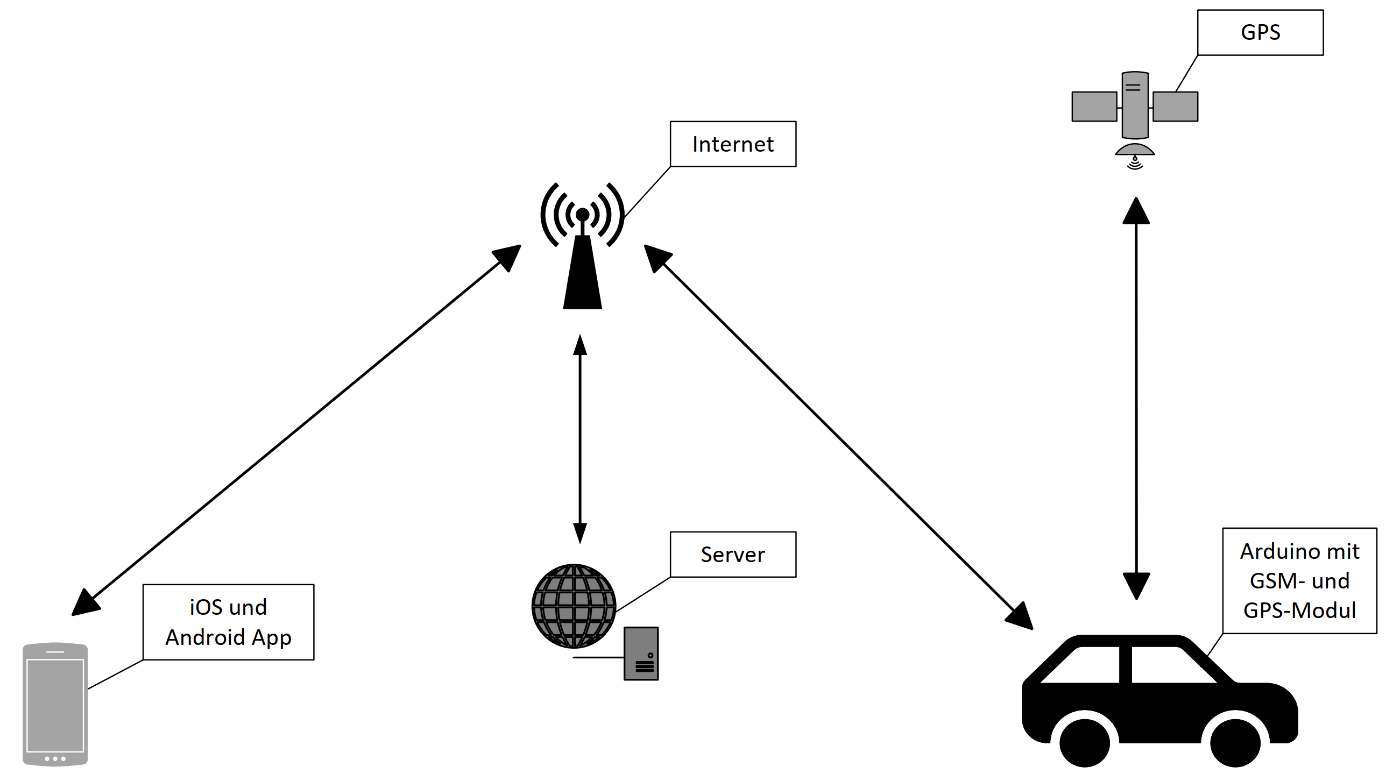
\includegraphics[width=1\textwidth]{Bilder/Konzept_Konzept.png}
		\caption{Systemkonzept}
		\label{konzept}
	\end{center}
\end{figure}
Im Fahrzeug wollen wir einen Arduino Uno zusammen mit einem passenden GSM- und GPS-Modul platzieren. Dieser ermittelt in bestimmten Zeitintervallen die aktuelle Position des Fahrzeugs und schickt die Koordinaten über die GSM-Verbindung an unseren Webserver. Dieser verarbeitet diese Daten und stellt sie anschließend so bereit, dass die Apps beider Betriebssysteme die aktuellen Koordinaten abfragen können.
